\section[\MakeUppercase{Materiais e Métodos}]{\texorpdfstring{\MakeUppercase{Materiais e Métodos}}{MATERIAIS E MÉTODOS}}\label{sec:materiais e métodos}

O aparato experimental consiste em um sistema de condicionamento de ar automotivo equipado com transdutores de pressão, temperatura e umidade relativa, vazão mássica e controle de temperatura com resistências elétricas, além de um sistema de aquisição de dados instalado na bancada de testes, destinado à execução de ensaios experimentais e à coleta de dados. Detalhes adicionais sobre a bancada experimental podem ser encontrados no relatório de \textcite{deoliveira2023} e no artigo de \textcite{dasilva2024}.

As atividades experimentais serão conduzidas no laboratório de refrigeração veicular, situado no campus Joinville da Universidade Federal de Santa Catarina \cite{reve2023}. Por sua vez, uma imagem real da bancada que será utilizada para a obtenção dos dados experimentais é apresentada na Figura \ref{fig:bancada de teste}.

\begin{figure}[ht]
    \centering
     \caption{Bancada Experimental}
    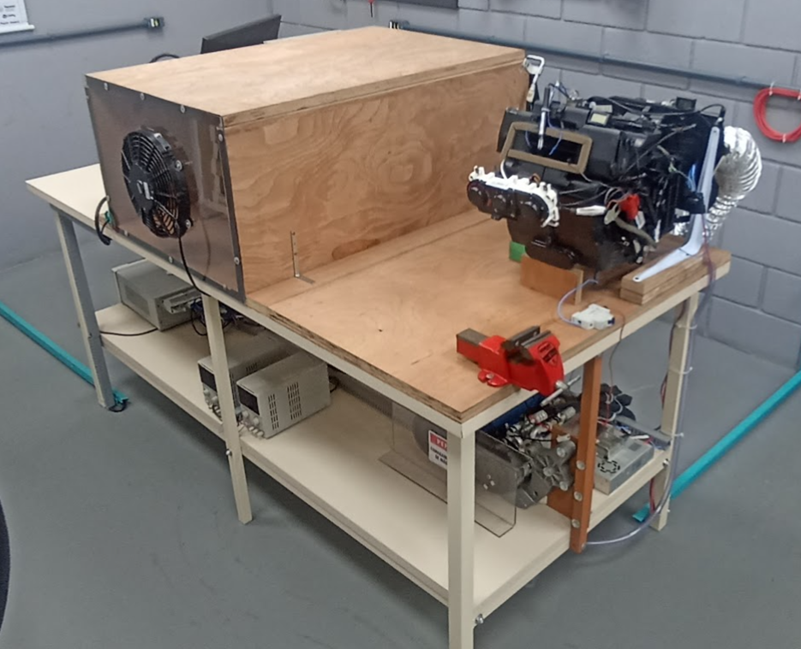
\includegraphics[width=13.56cm, height=10.99cm]{FigurasdoTexto/Bancada Experimental.png}
    \vspace{5pt}  % Add space before source
    
    {\footnotesize Fonte: O Autor (2024)}  % Source text in smaller font
    \label{fig:bancada de teste}
\end{figure}
\newpage
Para a coleta de dados, foram instalados transdutores em pontos específicos no sistema de condicionamento de ar, com 17 transdutores de temperatura, 2 transdutores de pressão, 2 transdutores de umidade relativa e 3 resistências para o controle de temperatura. As posições dos pontos de medição das propriedades do sistema estão presentes na Figura \ref{fig:instalação transdutores}. 

\begin{figure}[ht]
    \centering
     \caption{Representação dos Pontos de Instalação dos Transdutores}
    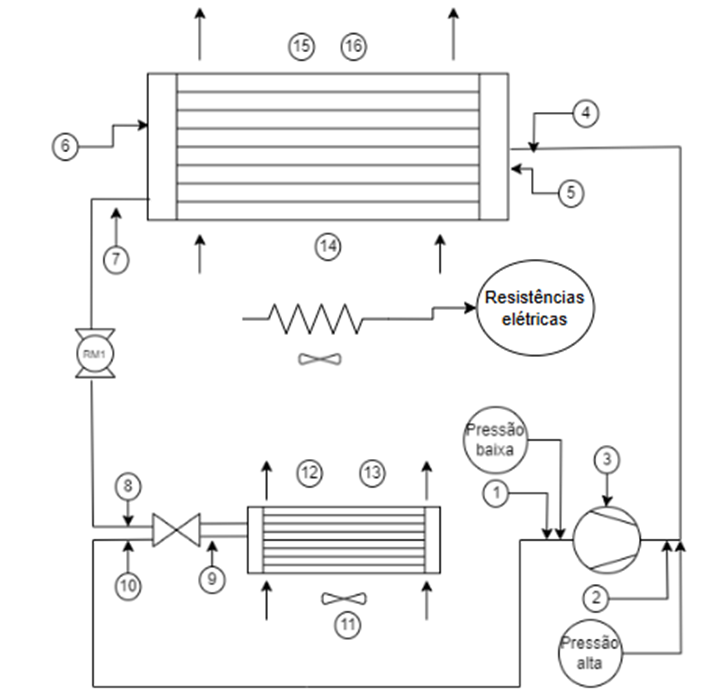
\includegraphics[width=11.75cm, height=11.88cm]{FigurasdoTexto/Instalação Transdutores.png}
    \vspace{5pt}  % Add space before source
    
    {\footnotesize Fonte: O Autor (2024)}  % Source text in smaller font
    \label{fig:instalação transdutores}
\end{figure}
\newpage
\subsection{PLANEJAMENTO EXPERIMENTAL}

O plano de teste foi desenvolvido com o objetivo de validar os dados obtidos pelo sistema de aquisição. Para a realização da fase experimental, foram elaborados dois roteiros para duas análises distintas: A primeira, que pode ser encontrada na Tabela \ref{tab:pertubaçõesTransiente}, tem o intuito único de analisar como diferentes perturbações causadas ao sistema afetam seu comportamento transiente. Os testes serão realizados alterando dois principais parâmetros: a frequência de rotação do compressor e a posição de velocidade do ventilador do evaporador.

\begin{table}[htb]
    \centering
    \begin{tabular}{|c|c|c|}
        \hline
        \textbf{Perturbação} & \makecell{\textbf{Frequência de Rotação do} \\ \textbf{Compressor Esperada [RPM]}} & \textbf{Posição Ventilador} \\
        \hline
        P1 & 500 & 1 $\rightarrow$ 4  \\
        P2 & 500 $\rightarrow$ 890 & 4  \\
        P3 & 890 & 4 $\rightarrow$ 1  \\
        \hline
    \end{tabular}
    \caption{Perturbações Geradas no Sistema de Refrigeração para Análise do Transiente}
    \vspace{5pt} 
{\footnotesize Fonte: O Autor (2025) }
    \label{tab:pertubaçõesTransiente}
\end{table}

Na segunda análise, o intuito principal muda. Pretende-se gerar uma perturbação ao sistema, esperar que ele entre em estado permanente e, então, voltar ao seu estado inicial, observando assim se existe histerese no sistema de refrigeração e, posteriormente, avaliando seu impacto. A Tabela \ref{tab:pertubaçõesHisterese} então mostra as perturbações causadas no sistema para a segunda parte deste trabalho. Apenas a frequência de rotação foi alterada, aumentando-a e depois voltando ao ponto original, mantendo a posição do ventilador fixa.
\\
\begin{table}[h]
    \centering
    \begin{tabular}{|c|c|c|}
        \hline
        \textbf{Perturbação} & \makecell{\textbf{Frequência de Rotação do} \\ \textbf{Compressor Esperada [RPM]}} & \textbf{Posição Ventilador} \\
        \hline
        P4 & 890 $\rightarrow$ 1074 & 4  \\
        P5 & 1074 $\rightarrow$ 890 & 4  \\
        \hline
    \end{tabular}
    \caption{Perturbações Geradas no Sistema de Refrigeração para Análise da Histerese}
    
    \vspace{5pt} 
    {\footnotesize Fonte: O Autor (2025)}
    \label{tab:pertubaçõesHisterese}
\end{table}

Para alterar a frequência de rotação do compressor, o laboratório \textcite{reve2023} tem à sua disposição um inversor CFW-300 da WEG conforme a Figura \ref{fig:inversor CFW-300}. O inversor controla a amplitude e frequência do sinal (em Hertz) de tensão alternada que chega até o motor trifásico, que é acoplado ao compressor através de uma embreagem eletromagnética. Este sinal de tensão com frequência diferente da rede elétrica é, então, responsável por controlar a velocidade de rotação do motor e, por consequência, do compressor. A variação da frequência pode ser facilmente alterada nos parâmetros do inversor e, com a ajuda de uma tabela experimental do laboratório, é possível saber a correspondência da frequência de rotação em Hertz do sinal gerado pela rotação do compressor em RPM.

\begin{figure}[h]
    \centering
    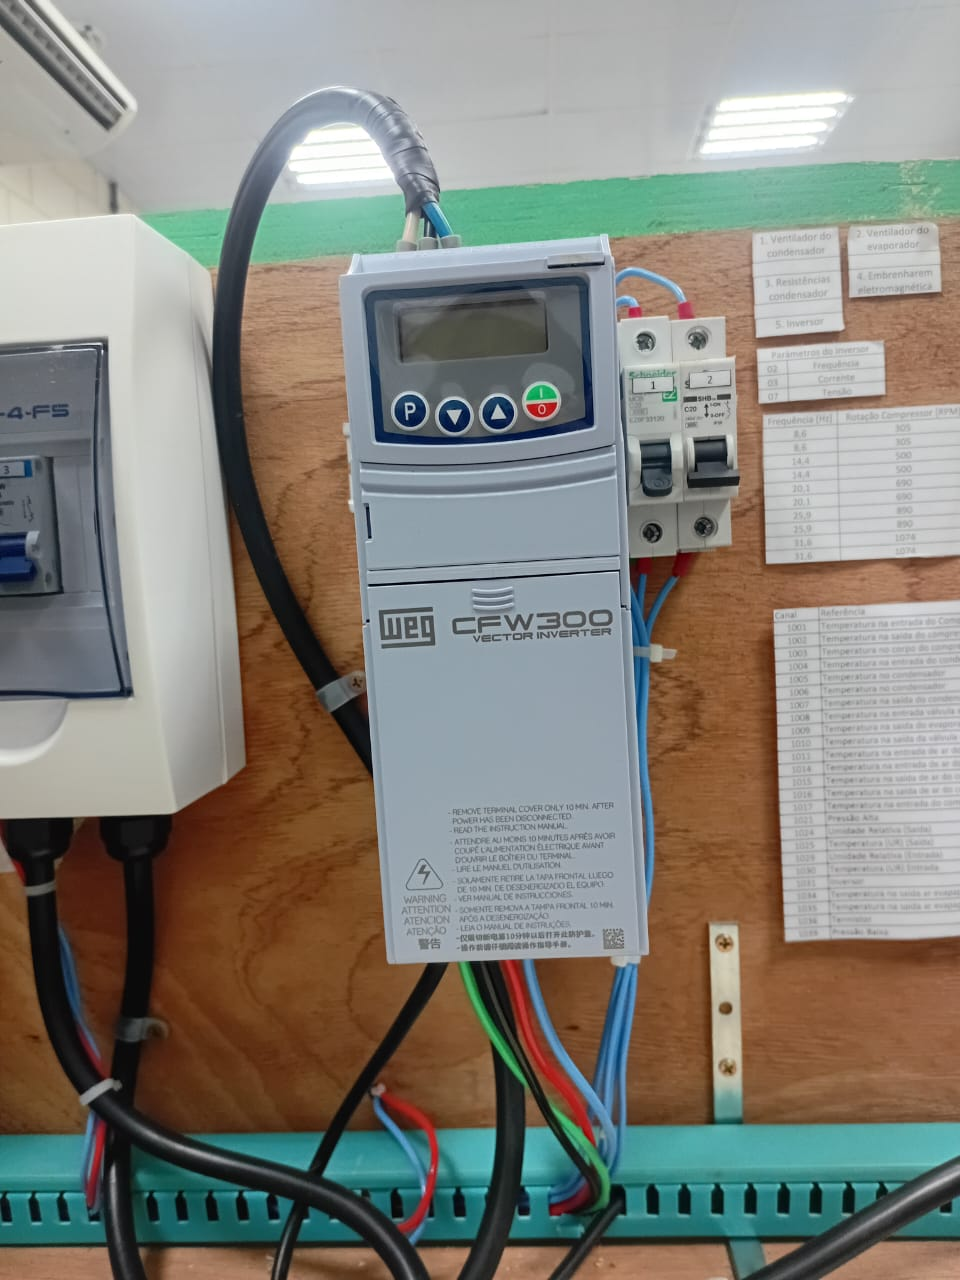
\includegraphics[width=0.45\linewidth]{FigurasdoTexto/inversorcfw-300.jpeg}
    \caption{Inversor CFW-300 Utilizado para Alterar a Velocidade de Rotação do Compressor}
    \label{fig:inversor CFW-300}
    {\footnotesize Fonte: O Autor (2025)}
\end{figure}

A posição do ventilador pode ser alterada em um painel analógico que é similar ao de muitos automóveis comerciais, como mostra a Figura \ref{fig:painelMudançadeVelocidadeVentilador}. É evidente que, diferentemente da frequência de rotação do compressor, o controle da vazão de ar do ventilador é menos preciso. A posição 0 representa o ventilador completamente desligado,enquanto as posições 1-4 representam um crescente de velocidade. A vazão de ar do ventilador nestas posições foi aferida em testes anteriores e estes dados estão inclusos no artigo de \textcite{ExperimentalThermalPerformance}.
\newpage
\begin{figure}[h]
    \centering
    \includegraphics[width=0.5\linewidth]{FigurasdoTexto/painelMudançadeVelocidadeVentilador.jpeg}
    \caption{Painel Utilizado para Alterar a Vazão de Ar do Ventilador do Evaporador}
    \label{fig:painelMudançadeVelocidadeVentilador}

    {\footnotesize Fonte: O Autor (2025)}

\end{figure}

\subsection{\MakeUppercase{Determinação dos Tempos de Acomodação do Sistema}} \label{subsec:Tempo de Acomodação do Sistema}

A determinação dos tempos de acomodação do sistema é importante para estudar o comportamento do sistema de refrigeração e, falar
 de forma mais assertiva sobre a diferença de convergência entre os testes de subida e descida de rotação do compressor, além de ser um parâmetro importante para possíveis modelos matemáticos que venham a ser desenvolvidos, por exemplo, para encontrar funções de transferência do sistema. 

Determinar estes valores não é uma tarefa trivial. Todavia, primeiro é preciso definir o conceito de tempo de acomodação. O tempo de acomodação, conforme \textcite{ogataControle} é o tempo necessário para que a curva de resposta do sistema alcance valores de, geralmente, 2\% ou 5\% do valor final. Para este trabalho, será utilizado o valor de 2\% do valor final, ou seja, o tempo de acomodação será definido como o tempo necessário para que a curva de resposta do sistema atinja 98\% do valor final.

Entretanto, como está sendo estudado um sistema real, é necessário levar em consideração principalmente o ruído dos dados experimentais. Caso este ruído não for levado em consideração, o valor do tempo de acomodação será calculado de forma errônea. Além disso, o transiente do sistema não inicia imediatamente na coleta de dados, os dados iniciais estão relacionados ao estado inicial permanente do sistema, portanto, ele não deve ser considerado no cálculo do tempo de acomodação. 

Assim, um algoritmo foi desenvolvido para calcular o tempo de acomodação do sistema. O algoritmo é o seguinte:

\begin{enumerate}   
    \item É calculado a média dos 10 primeiros valores do teste, estes valores serão utilizados como o valor inicial do sistema.
    \item É calculado a média dos últimos 10 valores do teste, estes valores serão utilizados como o valor final do sistema.
    \item Para filtrar os dados experimentais e diminuir o ruído, é aplicado um filtro de média móvel com janela de 10 amostras dos dados experimentais, suavizando assim a curva.
    \item Para detectar o início do transiente, é definido que o seu início no momento em que o valor da curva de resposta do sistema é maior ou menor que 2\% do valor inicial do sistema. O tempo aferido nesta amostra é o momento zero do cálculo do tempo de acomodação.
    \item O valor do tempo de acomodação do sistema será encontrado então a partir do último valor do teste, o tempo aferido na primeira amostra que for 2\% maior ou menor que o valor final do sistema (dependendo se a curva de resposta é crescente ou decrescente).
    \item O tempo de acomodação é então calculado como a diferença entre o tempo da amostra final e o tempo da amostra inicial do transiente.
\end{enumerate}

Um bom exemplo de como o algoritmo funciona é apresentado na Figura \ref{fig:exemplo de cálculo do tempo de acomodação}. É possível observar que, ao suavizar a curva, o algoritmo consegue detectar o início e fim do transiente e o tempo de acomodação do sistema, assim como os demais passos necessários para o cálculo de maneira coerente. Através do tempo de acomodação, é possível também definir as constantes de tempo do sistema, para sistemas de primeira ordem, a constante de tempo é definida como o tempo de acomodação dividido por 4 \cite{ogataControle}. Isto será relevante, já que boa parte das variáveis deste sistema, como será visto posteriormente, são, em boa aproximação, de primeira ordem.

\begin{figure}[h]
    \centering
    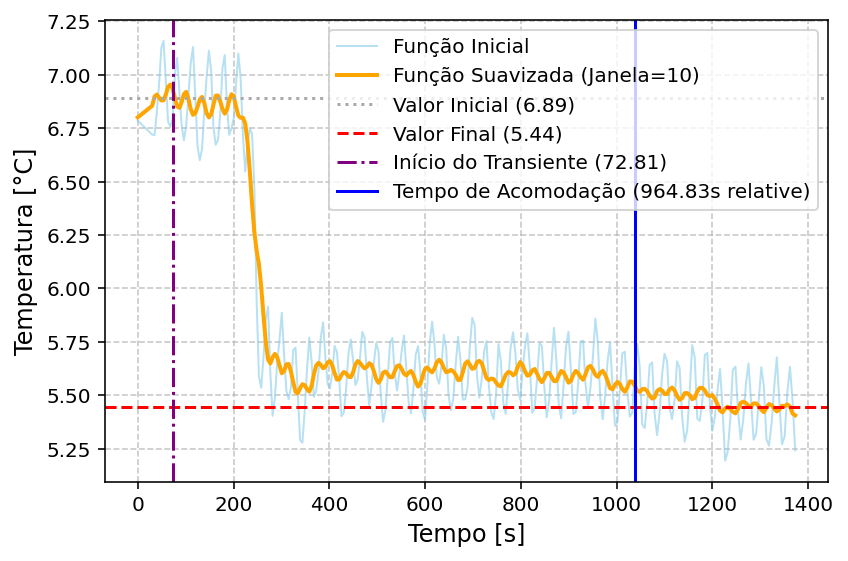
\includegraphics[width=1\linewidth]{FigurasdoTexto/Exemplo tempo de acomodação.png}
    \caption{Representação Visual do Algoritmo de Cálculo do Tempo de Acomodação}
    \label{fig:exemplo de cálculo do tempo de acomodação}
    {\footnotesize Fonte: O Autor (2025)}
\end{figure}
\subsection{\MakeUppercase{Análise e Comparação das Histereses}} \label{subsec:Método de Análise da Histerese}

Antes de realizar as análises em si, é preciso definir uma forma de comparar a histerese de várias variáveis diferentes de forma única. A histerese é usualmente definida como a área entre as curvas de subida e descida,isto é, a diferença de caminho entre a ida e volta a um mesmo ponto. A fim de ser possível relacionar diferentes variáveis com variações distintas, a histerese será calculada da seguinte forma: é feito o cálculo da diferença entre a área das curvas de subida e descida da velocidade de rotação do compressor, então esta área é dividida pela multiplicação dos intervalos das variáveis nos eixos t e y a fim de normalizá-la; por fim, é aplicado o módulo neste número. De forma genérica pode-se escrever a fórmula utilizada para o cálculo da histerese normalizada $\text{H}_\text{norm}$ como:

\begin{equation}
    H_{norm} = \abs*{{\frac{\int_{t_0} ^t  f_{subida}(t) dt - \int_{t_0} ^t  f_{descida}(t) dt   }{\Delta y\Delta t }}}
    \label{eq:histerese normalizada}
\end{equation}
\\
Em que t representa o tempo do teste, e as funções genéricas $f$ podem representar: temperatura, pressão ou vazão de fluido refrigerante. No entanto, como estas funções de ida e da volta na equação \ref{eq:histerese normalizada} são desconhecidas, dada a natureza do estudo experimental, estas integrais são calculadas de forma numérica utilizando o método numérico de 1/3 de Simpson composto \cite{ChapraNumerico}. Uma representação visual do que a equação \ref{eq:histerese normalizada} representa é apresentada na Figura \ref{fig:representação visual da histerese normalizada}, as funções $f_{subida}(t)$ e $f_{descida}(t)$ são representadas pelas curvas não tracejadas e o retângulo tracejado representa a área $\Delta y \Delta t$. Ao encontrar a área entre as duas curvas e dividi-la pela área do retângulo em que elas estão inscritas, encontra-se a porcentagem de histerese de determinada variável.

\begin{figure}[h]
    \centering
    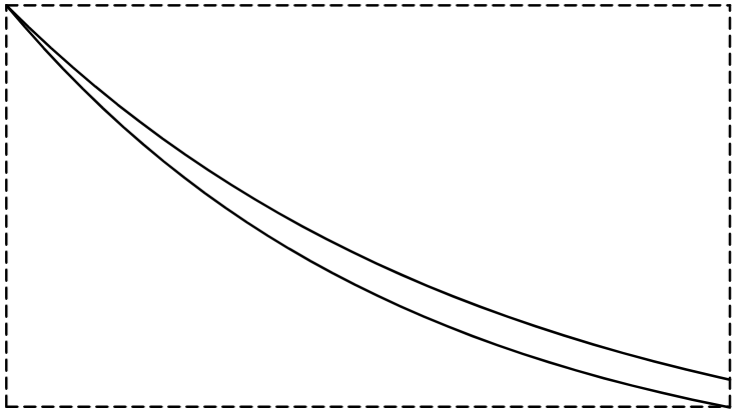
\includegraphics[width=0.75\linewidth]{FigurasdoTexto/Representação visual da histerese.png}
    \caption{Representação Visual da Histerese Normalizada}
    \label{fig:representação visual da histerese normalizada}
    {\footnotesize Fonte: O Autor (2025)}
\end{figure}


\subsection{\MakeUppercase{Determinação do COP do Sistema}} \label{subsec:Determinação do COP do Sistema}

O COP segue alguns dos métodos e dados experimentais já utilizados e existentes no laboratório \textcite{reve2023}, como no artigo de \textcite{ExperimentalThermalPerformance} no qual já constam dados experimentais da taxa de transferência de massa necessária para calcular o COP nas condições deste artigo. Isto é, o COP será avaliado da seguinte forma:

\begin{equation}
    COP = \frac{\dot Q_e}{\dot W}
    \label{eq:COP}
\end{equation}

Em que $\dot W$ é o consumo de potência do compressor e $ \dot Q_e$ é a capacidade de refrigeração do evaporador dada por:

\begin{equation}
    \dot Q_e = \dot m_{ar}(h_{ar,entrada} - h_{ar,saída})
\end{equation}

Em que $\dot m_{ar}$ é a taxa de transferência de massa de ar e $h_{ar}$ é a entalpia do ar úmido. O valor de $\dot m_{ar}$ será definido como 0,058 kg/s, dados experimentais provenientes do artigo de \textcite{ExperimentalThermalPerformance}. Os dados de entalpia são determinados utilizando o software ESS, para o cálculo das entalpias de entrada, os dados experimentais da temperatura e umidade relativa de entrada do evaporador foram utilizados, assumindo pressão constante igual a uma atmosfera. Para as entalpias de saída, foi também assumida uma pressão constante de uma atmosfera e utilizado os dados de temperatura e umidade relativa de saída do evaporador. 